% Generated by Listas/make_statements.py from pratica-lecture-08.md, item 20. Do not edit.
\textbf{Source.} Tadelis (2013), \emph{Game Theory: An Introduction}, Exercise 15.6 ``Selten's Horse'', p.~317 {[}PDF p.~336{]}. Reproduced verbatim. Answer: none in the book.



\begin{quote}

\textbf{Selten's Horse:} Consider the three-person game described in Figure 15.6, known as Selten's horse (for the obvious reason).



\pandocbounded{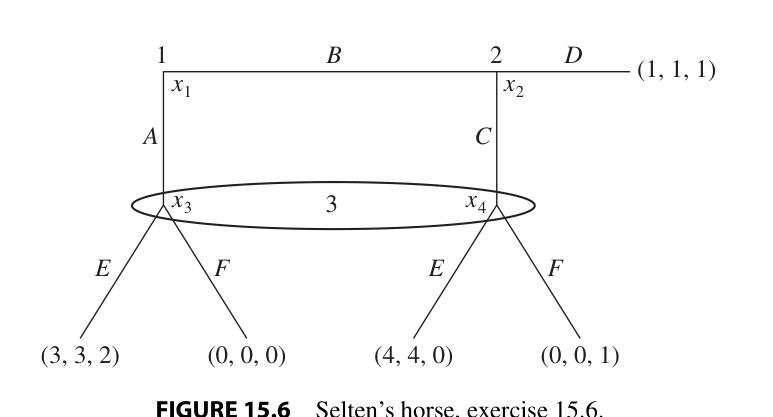
\includegraphics[keepaspectratio,alt={Figure 15.6 Selten's horse}]{../figures/tadelis-15-6.png}}



\textbf{FIGURE 15.6} Selten's horse, exercise 15.6.



\begin{enumerate}

\def\labelenumi{\alph{enumi}.}

\item

  What are the pure-strategy Bayesian Nash equilibria of this game?

\item

  Which of the Bayesian Nash equilibria that you found in (a) are perfect Bayesian equilibria?

\item

  Which of the Bayesian Nash equilibria that you found in (a) are sequential equilibria?

\end{enumerate}

\end{quote}

